\documentclass[journal,12pt,twocolumn]{IEEEtran}
%
\usepackage{setspace}
\usepackage{gensymb}
\usepackage{xcolor}
\usepackage{caption}
%\usepackage{subcaption}
%\doublespacing
\singlespacing

%\usepackage{graphicx}
%\usepackage{amssymb}
%\usepackage{relsize}
\usepackage[cmex10]{amsmath}
\usepackage{mathtools}
%\usepackage{amsthm}
%\interdisplaylinepenalty=2500
%\savesymbol{iint}
%\usepackage{txfonts}
%\restoresymbol{TXF}{iint}
%\usepackage{wasysym}
\usepackage{hyperref}
\usepackage{amsthm}
\usepackage{mathrsfs}
\usepackage{txfonts}
\usepackage{stfloats}
\usepackage{cite}
\usepackage{cases}
\usepackage{subfig}
%\usepackage{xtab}
\usepackage{longtable}
\usepackage{multirow}
%\usepackage{algorithm}
%\usepackage{algpseudocode}
%\usepackage{enumerate}
\usepackage{enumitem}
\usepackage{mathtools}
%\usepackage{iithtlc}
%\usepackage[framemethod=tikz]{mdframed}
\usepackage{listings}


%\usepackage{stmaryrd}


%\usepackage{wasysym}
%\newcounter{MYtempeqncnt}
\DeclareMathOperator*{\Res}{Res}
%\renewcommand{\baselinestretch}{2}
\renewcommand\thesection{\arabic{section}}
\renewcommand\thesubsection{\thesection.\arabic{subsection}}
\renewcommand\thesubsubsection{\thesubsection.\arabic{subsubsection}}

\renewcommand\thesectiondis{\arabic{section}}
\renewcommand\thesubsectiondis{\thesectiondis.\arabic{subsection}}
\renewcommand\thesubsubsectiondis{\thesubsectiondis.\arabic{subsubsection}}

%\renewcommand{\labelenumi}{\textbf{\theenumi}}
%\renewcommand{\theenumi}{P.\arabic{enumi}}

% correct bad hyphenation here
\hyphenation{op-tical net-works semi-conduc-tor}

\lstset{
language=Python,
frame=single, 
breaklines=true,
columns=fullflexible
}



\begin{document}
%

\theoremstyle{definition}
\newtheorem{theorem}{Theorem}[section]
\newtheorem{problem}{Problem}
\newtheorem{proposition}{Proposition}[section]
\newtheorem{lemma}{Lemma}[section]
\newtheorem{corollary}[theorem]{Corollary}
\newtheorem{example}{Example}[section]
\newtheorem{definition}{Definition}[section]
%\newtheorem{algorithm}{Algorithm}[section]
%\newtheorem{cor}{Corollary}
\newcommand{\BEQA}{\begin{eqnarray}}
\newcommand{\EEQA}{\end{eqnarray}}
\newcommand{\define}{\stackrel{\triangle}{=}}

\bibliographystyle{IEEEtran}
%\bibliographystyle{ieeetr}

\providecommand{\nCr}[2]{\,^{#1}C_{#2}} % nCr
\providecommand{\nPr}[2]{\,^{#1}P_{#2}} % nPr
\providecommand{\mbf}{\mathbf}
\providecommand{\pr}[1]{\ensuremath{\Pr\left(#1\right)}}
\providecommand{\qfunc}[1]{\ensuremath{Q\left(#1\right)}}
\providecommand{\sbrak}[1]{\ensuremath{{}\left[#1\right]}}
\providecommand{\lsbrak}[1]{\ensuremath{{}\left[#1\right.}}
\providecommand{\rsbrak}[1]{\ensuremath{{}\left.#1\right]}}
\providecommand{\brak}[1]{\ensuremath{\left(#1\right)}}
\providecommand{\lbrak}[1]{\ensuremath{\left(#1\right.}}
\providecommand{\rbrak}[1]{\ensuremath{\left.#1\right)}}
\providecommand{\cbrak}[1]{\ensuremath{\left\{#1\right\}}}
\providecommand{\lcbrak}[1]{\ensuremath{\left\{#1\right.}}
\providecommand{\rcbrak}[1]{\ensuremath{\left.#1\right\}}}
\theoremstyle{remark}
\newtheorem{rem}{Remark}
\newcommand{\sgn}{\mathop{\mathrm{sgn}}}
%\providecommand{\abs}[1]{\left\vert#1\right\vert}
\providecommand{\res}[1]{\Res\displaylimits_{#1}} 
\providecommand{\norm}[1]{\lVert#1\rVert}
\providecommand{\mtx}[1]{\mathbf{#1}}
%\providecommand{\mean}[1]{E\left[ #1 \right]}
\providecommand{\fourier}{\overset{\mathcal{F}}{ \rightleftharpoons}}
\providecommand{\ztrans}{\overset{\mathcal{Z}}{ \rightleftharpoons}}

%\providecommand{\hilbert}{\overset{\mathcal{H}}{ \rightleftharpoons}}
\providecommand{\system}{\overset{\mathcal{H}}{ \longleftrightarrow}}
	%\newcommand{\solution}[2]{\textbf{Solution:}{#1}}
\newcommand{\solution}{\noindent \textbf{Solution: }}
\providecommand{\dec}[2]{\ensuremath{\overset{#1}{\underset{#2}{\gtrless}}}}
\numberwithin{equation}{section}
%\numberwithin{equation}{subsection}
%\numberwithin{problem}{subsection}
%\numberwithin{definition}{subsection}
\makeatletter
\@addtoreset{figure}{problem}
\makeatother

\let\StandardTheFigure\thefigure
%\renewcommand{\thefigure}{\theproblem.\arabic{figure}}
\renewcommand{\thefigure}{\theproblem}


%\numberwithin{figure}{subsection}

\def\putbox#1#2#3{\makebox[0in][l]{\makebox[#1][l]{}\raisebox{\baselineskip}[0in][0in]{\raisebox{#2}[0in][0in]{#3}}}}
     \def\rightbox#1{\makebox[0in][r]{#1}}
     \def\centbox#1{\makebox[0in]{#1}}
     \def\topbox#1{\raisebox{-\baselineskip}[0in][0in]{#1}}
     \def\midbox#1{\raisebox{-0.5\baselineskip}[0in][0in]{#1}}

\vspace{3cm}

\title{ 
%\logo{
Introduction to Bayesian Statistics\\
Real Data Analysis
%}
%	\logo{Octave for Math Computing }
}
%\title{
%	\logo{Matrix Analysis through Octave}{\begin{center}\includegraphics[scale=.24]{tlc}\end{center}}{}{HAMDSP}
%}

% paper title
% can use linebreaks \\ within to get better formatting as desired
%\title{Matrix Analysis through Octave}
%
%
% author names and IEEE memberships
% note positions of commas and nonbreaking spaces ( ~ ) LaTeX will not break
% a structure at a ~ so this keeps an author's name from being broken across
% two lines.
% use \thanks{} to gain access to the first footnote area
% a separate \thanks must be used for each paragraph as LaTeX2e's \thanks
% was not built to handle multiple paragraphs
%

\author{ Anita Dash-MA20BTECH11001 \quad
Krishna Teja-MA20BTECH11005 \\
KN Vardhan-MA20BTECH11006 }

% note the % following the last \IEEEmembership and also \thanks - 
% these prevent an unwanted space from occurring between the last author name
% and the end of the author line. i.e., if you had this:
% 
% \author{....lastname \thanks{...} \thanks{...} }
%                     ^------------^------------^----Do not want these spaces!
%
% a space would be appended to the last name and could cause every name on that
% line to be shifted left slightly. This is one of those "LaTeX things". For
% instance, "\textbf{A} \textbf{B}" will typeset as "A B" not "AB". To get
% "AB" then you have to do: "\textbf{A}\textbf{B}"
% \thanks is no different in this regard, so shield the last } of each \thanks
% that ends a line with a % and do not let a space in before the next \thanks.
% Spaces after \IEEEmembership other than the last one are OK (and needed) as
% you are supposed to have spaces between the names. For what it is worth,
% this is a minor point as most people would not even notice if the said evil
% space somehow managed to creep in.



% The paper headers
%\markboth{Journal of \LaTeX\ Class Files,~Vol.~6, No.~1, January~2007}%
%{Shell \MakeLowercase{\textit{et al.}}: Bare Demo of IEEEtran.cls for Journals}
% The only time the second header will appear is for the odd numbered pages
% after the title page when using the twoside option.
% 
% *** Note that you probably will NOT want to include the author's ***
% *** name in the headers of peer review papers.                   ***
% You can use \ifCLASSOPTIONpeerreview for conditional compilation here if
% you desire.




% If you want to put a publisher's ID mark on the page you can do it like
% this:
%\IEEEpubid{0000--0000/00\$00.00~\copyright~2007 IEEE}
% Remember, if you use this you must call \IEEEpubidadjcol in the second
% column for its text to clear the IEEEpubid mark.



% make the title area
\maketitle

%\newpage

\tableofcontents

%\renewcommand{\thefigure}{\thesection.\theenumi}
%\renewcommand{\thetable}{\thesection.\theenumi}

\renewcommand{\thefigure}{\theenumi}
\renewcommand{\thetable}{\theenumi}

%\renewcommand{\theequation}{\thesection}


\bigskip

% \section{Software Installation}
% Run the following commands
% \begin{lstlisting}
% sudo apt-get update
% sudo apt-get install libffi-dev libsndfile1 python3-scipy  python3-numpy python3-matplotlib 
% sudo pip install cffi pysoundfile 
% \end{lstlisting}
\begin{abstract}
% Here, the abstract
This report is based on a group project part of the MA4740
- Introduction to Bayesian Statistics course material. The primary
goal of this project is to acquire a real-world data set (not
synthetic) and execute Beta Binomial Bayesian Analysis and
other approaches presented in class..
\end{abstract}
\section{Introduction}
The project includes collecting a real-life data set and applying the statistical methods while also performing a beta-binomial bayesian analysis. The real-life data set that we have taken is based on the stocks of MSFT (Microsoft Corp) from the past 2000 to 2022, for the prior dataset. \\

The real-life data set, MSFT stocks have been taken from the Python3 \textit{yfinance} package. The data includes opening price, closing price, maximum price, minimum price and date. Amongst which, the attributes that are of our interest are closing price and date.

\section{Prior Data}
 The prior data is on the stocks of MSFT from the year 2000 to 2022. The closing price of MSFT stocks on each day throughout the years is considered. Based on this prior data, we attempt to predict if MSFT’s stock
will rise or fall on a specific day after 2022. \\

The Prior Dataset is made up of the fraction of stock increases in each quarter from year 2000 to 2022.If the stock has increased from the previous day, the value is 1, otherwise it is 0. We choose a random variable X , where X is the proportion of days the stock price increased in n days, and P(X = x)
representing the probability of the proportion, x \\

\textbf{E.g.} Suppose in the past $n$ days, the MSFT stock has increased $k$ times, then
\begin{equation}
    x = \frac{k}{n}
\end{equation}

The plot between these proportions with its frequency gives us a near normal distribution. This is our prior data and it's probability mass function has been depicted below.
\begin{figure}[!ht]
\centering
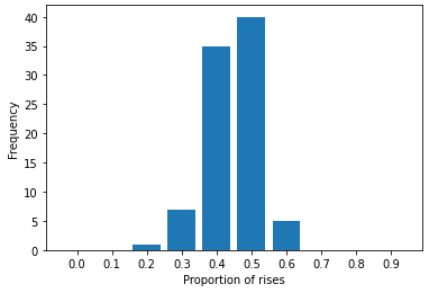
\includegraphics[width=\columnwidth]{Images/FreqVsRise.png}
\end{figure}
\section{Applying the Methods}
We apply MOM and MLE to fit the normal distribution of our prior data.\\
We know That,

\begin{equation}
    E[X] = \mu = \frac{1}{n}\Sigma x_{i}
\end{equation}

\begin{equation}
    E[X^2] = \mu^2 + \sigma^2 = \frac{1}{n}\Sigma x_{i}^{2}
\end{equation}

where, \\
$x_i$ are i.i.d realized values of $X$ and \\
$N(\mu,\sigma)$ is the normal distribution that fits the prior data.
\\

Since our distribution is a normal distribution, the MOM and MLE yield the same result. Below is the plot depicted for MOM and MLE.
\begin{figure}[!ht]
\centering
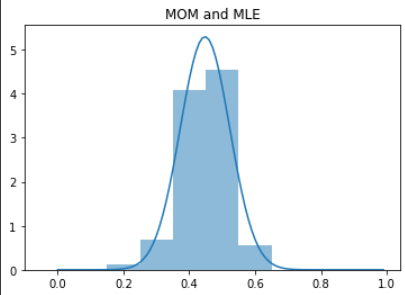
\includegraphics[width=\columnwidth]{Images/MOM_MLE.png}
\end{figure}

\section{Beta Distribution}
We try to fit the prior data distribution to a beta distribution.\newline
In a beta distribution, we get $X \sim Beta(\alpha, \beta)$, where,
\begin{equation}
    mean = \frac{\alpha}{\alpha + \beta}
\end{equation}
\begin{equation}
     var = \frac{\alpha\beta}{(\alpha + \beta)^2(\alpha + \beta + 1)}
\end{equation}
The calculations yield us the results
\begin{center}
First moment = Mean ($\mu$) = 0.4647727,\\
Second moment = 0.2235227,\\
Variance = 0.0075090,\\
Standard Deviation = 0.08665477,\\
\end{center}
And the values of $\alpha$, $\beta$ are 19.055, 23.504 respectively.
Given below is the plot of pdf of beta distribution of the prior data.
\begin{figure}[!ht]
\centering
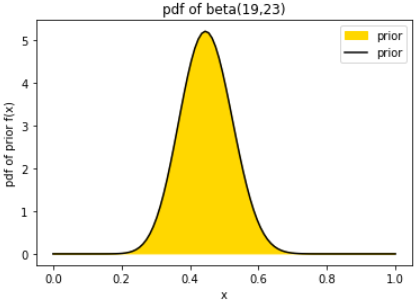
\includegraphics[width=\columnwidth]{Images/Pdf_beta_prior.png}
\label{fig:yndft}
\end{figure}
\section{Data-Likelihood Function}
Now we require a likelihood function to perform a beta-binomial analysis on the generated beta distribution.\\
We choose $L \mid \pi \sim Bin(n,\pi)$ where,
\begin{center}
    $n$: Number of days we are checking if the stock prize increased or decreased \\
    $\pi$: Probability of stock getting increased
\end{center}
the Data consists of the realized proportion of increase in stocks in the year 2022, where
\begin{center}
    n = 251 \\
y = 116 \\
p = 0.46215
\end{center}
 And the plot of the likelihood function and the prior distributions are  as follows
\begin{figure}[!ht]
\centering
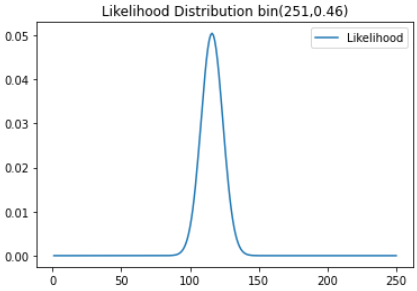
\includegraphics[width=\columnwidth]{Images/Likelihood_Dist.png}
\label{fig:yndft}
\end{figure}

\begin{figure}[!ht]
\centering
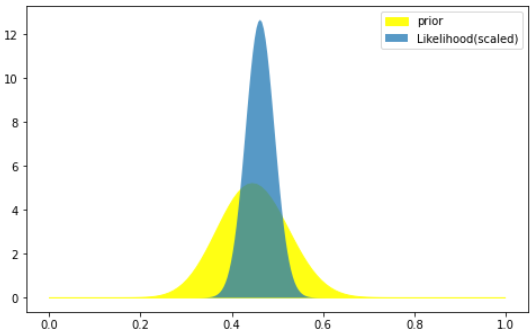
\includegraphics[width=\columnwidth]{Images/Prior_Likelihood.png}
\label{fig:yndft}
\end{figure}
\section{Posterior Distribution}
We find the posterior distribution by using the prior data and the likelihood function. \\
In a posterior distribution, we have,
\begin{equation}
\pi \mid L = y \sim beta(\alpha', \beta')
\end{equation}
where, 
\begin{center}
$\alpha' = \alpha + y$, \\
$\beta' =  \beta + n - y$ \\ 
\end{center}
 
$y$ is the realized value of number of times stocks increased in $n$ days


Thus, after performing the necessary calculations, we get 
\begin{center}
posterior alpha = 135.0546860782528\\
posterior beta = 158.50400363967225\\
Posterior mean = 0.46006025646191656\\    
\end{center}

And the plot is as shown below
\begin{figure}[!ht]
\centering
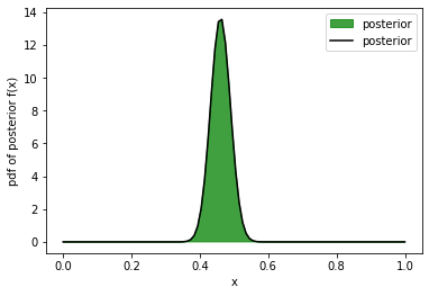
\includegraphics[width=\columnwidth]{Images/Posterior_Dist.png}
\caption{Posterior Distribution}
\label{fig:yndft}
\end{figure}
\section{Conclusion}
From the below combined plot we can see that the mean of our prior and posterior differ by 0.02 which is not that high. But the variance of prior and posterior differ.

        \begin{align*}
        \textit{Prior std} = 0.07534356570114019\\
        \textit{Post std} = 0.029039831153004316
        \end{align*}

        \begin{align*}
        \textit{Prior estimation of proportion} \approx \left (29.704\%, 59.841\% \right )\\
        \textit{Posterir estimation of proportion} \approx \left (40.198\%, 51.813\% \right )
        \end{align*}
\begin{figure}[!ht]
\centering
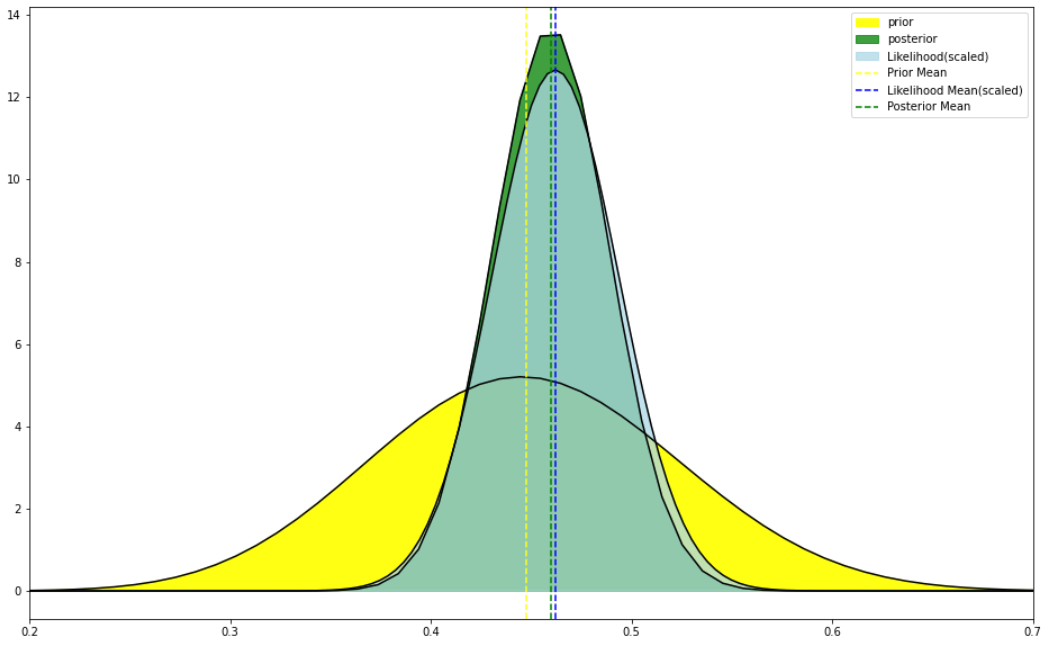
\includegraphics[width=\columnwidth]{Images/Final_Comb_Plot.png}
\caption{Combined Plot}
\label{fig:yndft}
\end{figure}
\begin{center}     \href{https://colab.research.google.com/drive/1AMuKl883Mes_bpji0VLkH9uxfi8i9bwj?usp=sharing}{\tobutton{Link-Source Code}}
\end{center}
\end{document}